\section{Results}
\label{section:results}

\subsection{Theoretical Results}
\label{subsection:theoretical_results}

\begin{theorem}
\label{thm:ARE}
For any $i$ and $j$, conditioning on $X_i = \nu_{\tau_i}$ and $X_j = \nu_{\tau_j}$, we have
\[
	\mathrm{ARE}(\bar{A}_{ij}, \hat{P}_{ij}) = 0.
\]
And for $N$ large enough, conditioning on $X_i = \nu_{\tau_i}$ and $X_j = \nu_{\tau_j}$, we have
\[
	\mathrm{RE}(\bar{A}_{ij}, \hat{P}_{ij}) \approx
    \frac{1/\rho_{\tau_i} + 1/\rho_{\tau_j}}{N}.
\]
\end{theorem}
This comes from a proof (outlined in section 5.6) for the variance of $\hat{P}_{ij}$ under the condition that N is large:
\begin{lemma}
\label{lm:VarPhat}
In the same setting as above, for any $i, j$, conditioning on $X_i = \nu_{\tau_i}$ and $X_j = \nu_{\tau_j}$, we have
\[
	\lim_{n \to \infty} N \cdot \mathrm{Var}(\hat{P}_{ij}) =
    \frac{1/\rho_{\tau_i} + 1/\rho_{\tau_j}}{M} P_{ij} (1 - P_{ij}).
\]
And for $N$ large enough, conditioning on $X_i = \nu_{\tau_i}$ and $X_j = \nu_{\tau_j}$, we have
\[
	E[(\hat{P}_{ij} - P_{ij})^2] \approx
    \frac{1/\rho_{\tau_i} + 1/\rho_{\tau_j}}{M N} P_{ij}(1-P_{ij}).
\]
\end{lemma}
Further, knowing that $\bar{A}_{ij}$ is the average of M samples from the Bernoulli distribution with parameter $P_{ij}$, the variance of $\bar{A}_{ij}$ should be $P_{ij}(1-P_{ij})/M$, which yields the above result.

This result implicates that for large random dot product graphs that follow a stochastic block model, a better estimate for the mean graph, under MSE, is the $\hat{P}$ estimate.


\subsection{Validation with Simulations}
\label{subsection:simulations}
We demonstrate the theoretical results in Section 3.1, the variance of $\hat{P}$ and the relative efficiency, via various Monte Carlo simulation experiments. Specifically, we consider the 2-block SBM parameterized by
\begin{equation*}
B = \begin{bmatrix}
0.42 & 0.2 \\
0.2 & 0.7
\end{bmatrix}
,\qquad \rho = \begin{bmatrix}
0.5 & 0.5
\end{bmatrix}.
\end{equation*}

The block proportion vector $\rho$ shows that each vertex is uniformly assigned to either block. And probability matrix $B$ indicates the probability of corresponding edges.

For each Monte Carlo replicate, we generate $M$ random graphs with known vertex correspondence under the SBM described above. Specifically, we first draw the block assignment $\tau \in [K]^N$ for each vertex from a multinomial distribution with parameter $\rho$. Note that $\tau$ will be identical for all $M$ graphs we are going to generate for vertex correspondence. Then we sample $M$ conditionally independent graphs $A^{(1)}, \cdots, A^{(M)}$, which are binary, symmetric and hollow, such that $A^{(m)}_{ij}|\tau \stackrel{ind}{\sim} Bern(P_{ij})$, where $P_{ij} = B_{\tau_i, \tau_j}$, $1 \le m \le M$, $1 \le i < j \le N$.

Given $M$ graphs, we can calculate $\bar{A}$ and $\hat{P}$ assuming that $d = \mathrm{rank}(B) = 2$ is known. Also, $\mathrm{MSE}(\hat{P}_{ij})$, $\mathrm{MSE}(\bar{A}_{ij})$ and $\mathrm{RE}(\bar{A}_{ij}, \hat{P}_{ij})$ with $1 \le i < j \le N$ for the data can be derived as $P$ is known in this simulation. Moreover, since vertices are equivalent in the same block under the SBM, we average over all the MSE and RE associated with edges corresponding to the same blocks as our estimates using the true labels $\tau$. That is, $\mathrm{MSE}_{st}(\hat{P}) = (\sum_{\tau_i = s, \tau_j = t, i\ne j} \mathrm{MSE}(\hat{P}_{ij}))/(\sum_{\tau_i = s, \tau_j = t, i\ne j}1)$, $\mathrm{MSE}_{st}(\bar{A}) = (\sum_{\tau_i = s, \tau_j = t, i\ne j} \mathrm{MSE}(\bar{A}_{ij}))/(\sum_{\tau_i = s, \tau_j = t, i\ne j}1)$ and $\mathrm{RE}_{st}(\bar{A}, \hat{P}) = \mathrm{MSE}_{st}(\hat{P})/\mathrm{MSE}_{st}(\bar{A})$ for $1 \le s, t \le K$.

By checking the averaging MSE and RE of the two estimates $\hat{P}$ and $\bar{A}$ over 1000 Monte Carlo replicates, we demonstrate that the theoretical results in Section \ref{subsection:theoretical_results}.

Figure \ref{fig:MSE} plots the scaled average MSE with different $N$ and $M$ of 1000 Monte Carlo replicates. Colors denote the block membership associated with the edges we are averaging over. Lines in black represent the theoretical values.
Figure \ref{fig:MSE}(a) shows that with a fixed $M$, as $N$ increases, $N \cdot \mathrm{MSE}_{st}(\hat{P})$ converges to $(1/\rho_s + 1/\rho_t) B_{st}(1-B_{st}) / M$ represented as the black lines, as suggested in Lemma \ref{lm:VarPhat}. Notice that this means $\mathrm{MSE}_{st}(\hat{P})$ is decreasing at rate $1/N$.
Figure \ref{fig:MSE}(b) illustrates that $M \cdot \mathrm{MSE}_{st}(\hat{P})$ holds to be $(1/\rho_s + 1/\rho_t) B_{st}(1-B_{st}) / N$ approximately independent of the value of $M$ while keeping $N$ sufficiently large and fixed. Thus a sufficiently large $M$ is not a necessary condition for Lemma \ref{lm:VarPhat} as expected.


\begin{figure}[!htb]
\centering
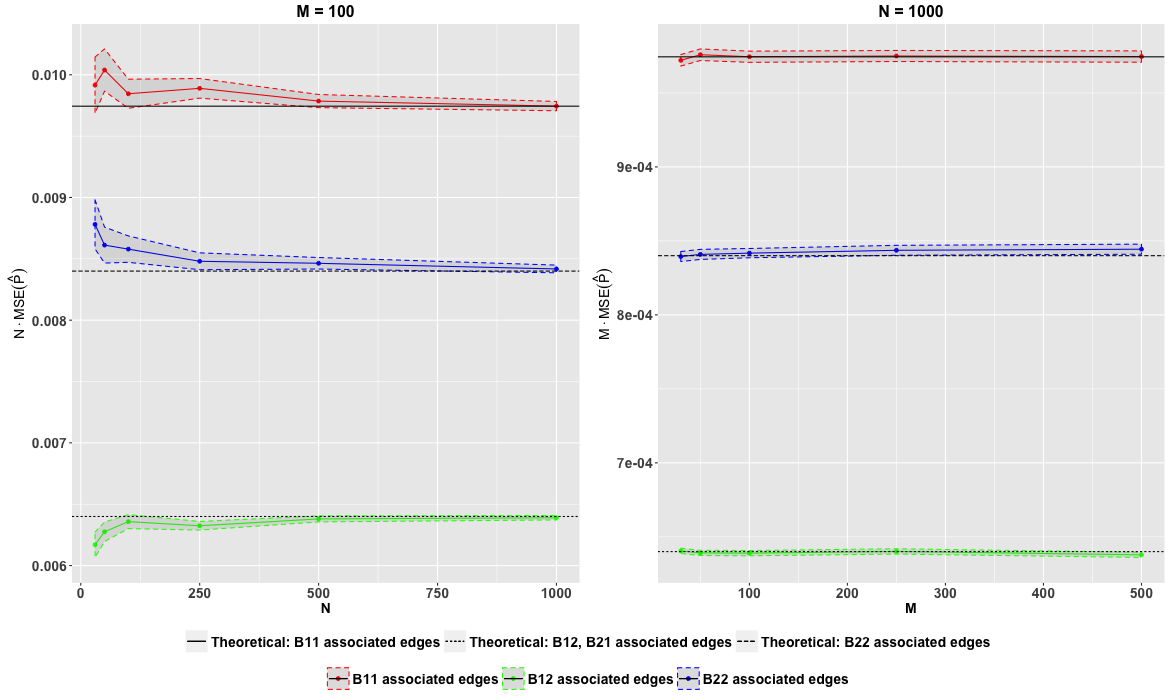
\includegraphics[width=16cm]{MSE.png}
\caption{Simulation results for the scaled average MSE of $\hat{P}$ with different $N$ and $M$ of 1000 Monte Carlo replicates. Colors denote the block membership associated with the edges we are averaging over. Lines in black represent the theoretical values.
 (a) shows that $N \cdot \mathrm{MSE}_{st}(\hat{P})$ converges to $(1/\rho_s + 1/\rho_t) B_{st}(1-B_{st}) / M$ represented as the dashed lines with a fixed $M$ as $N$ increases.
 (b) illustrates that $M \cdot \mathrm{MSE}_{st}(\hat{P})$ holds to be $(1/\rho_s + 1/\rho_t) B_{st}(1-B_{st}) / N$ approximately independent of the value of $M$ while keeping $N$ sufficiently large and fixed.}
\label{fig:MSE}
\end{figure}




Figure \ref{fig:RE} plot the scaled average RE with different $N$ and fixed $M$ of 1000 Monte Carlo replicates. Colors denote the block membership associated with the edges we are averaging over. Solid line in black represents the theoretical value for scaled RE. From the figure, we see that $N \cdot \mathrm{RE}_{st}(\bar{A}, \hat{P})$ converges to $1/\rho_s + 1/\rho_t$ represented as the black solid line, as suggested in Lemma \ref{thm:ARE}. Notice that this means $\mathrm{RE}_{st}(\bar{A}, \hat{P})$ is decreasing at rate $1/N$.


\begin{figure}[!htb]
	\centering
	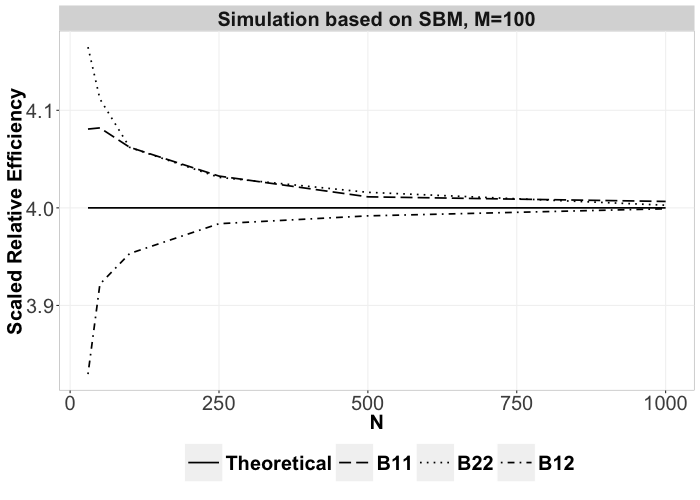
\includegraphics[width=9cm]{RE.png}
	\caption{Scaled average RE with different $N$ and fixed $M$ of 1000 Monte Carlo replicates. Solid line in black represents the theoretical value for scaled RE. Observe that $N \cdot \mathrm{RE}_{st}(\bar{A}, \hat{P})$ converges to $1/\rho_s + 1/\rho_t$ as expected.}
	\label{fig:RE}
\end{figure}




To verify Theorem \ref{thm:ARE} and Lemma \ref{lm:VarPhat} holds with different $\rho$, Figure \ref{fig:RErho} shows the average MSE and average RE with $N = 500$ and $M = 100$ while changing $\rho_1$ from 0.1 to 0.9. These simulated results again match well for the predictions from Theorem \ref{thm:ARE} and Lemma \ref{lm:VarPhat}.
\begin{figure}[!htb]
\centering
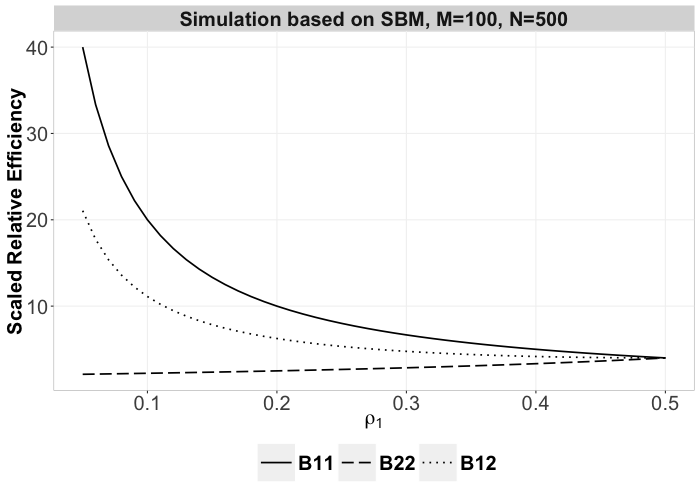
\includegraphics[width=14cm]{Rho.png}
\caption{Simulated results for (a) $\mathrm{MSE}_{st}(\hat{P})$ and (b) $\mathrm{RE}_{st}(\bar{A}, \hat{P})$ with $N = 500$ and $M = 100$ of 1000 Monte Carlo replicates while changing $\rho_1$ from 0.1 to 0.9.. The simulated values for the average MSE and average RE measurements match perfectly with the theoretical values.}
\label{fig:RErho}
\end{figure}





\subsection{CoRR Brain Graphs}
\label{subsection:real_data}

To demonstrate that the $\hat{P}$ estimate is valid under data that does not perfectly follow a SBM, we examine three datasets, JHU, desikan and CPAC200, which are sets of 454 brain connectomes with different number of nodes generated from fMRI scans available at the Consortium for Reliability and Reproducibility (CoRR). Details on these datasets and connectome generation can be seen in Section \ref{subsection:data_description}.  The connectomes generated have 48(JHU), 70(desikan) and 200(CPAC200) vertices respectively, with anatomical correspondence. To compare $\bar{A}$ and $\hat{P}$ we perform a cross-validation study to examine the impact of the number of available graphs $M$.  For each sample size $M$, we randomly sample $M$ graphs from the 454 graphs in the CoRR dataset and estimate the mean with both $\bar{A}$ and $\hat{P}$ with some proper embedding dimension.  Also, we assure $M$ to be relatively small such that the mean of the $(454 - M)$ remaining graphs is a valid approximation to the true probability matrix $P$ we are estimating. Then we can calculate the MSE of the two estimators based on the estimated probability matrix similarly as long as we know which dimension we should embed the graphs into.

Figure \ref{fig:JHU}, Figure \ref{fig:desikan} and Figure \ref{fig:CPAC200} demonstrate that when $M$ is small, $\hat{P}$ estimate outperforms $\bar{A}$ in MSE when applying our algorithm to the three datasets. As we can see, Zhu and Ghodsi's algorithm does a good job on these datasets. Moreover, the result is insensitive to the embedding dimension we choose, which makes our estimator more robust and useful in analyzing real data. The results justify that $\hat{P}$ is a valid and likely more accurate estimate of $P$ even when the data does not perfectly follow an SBM.

\begin{figure}[!htb]
\centering
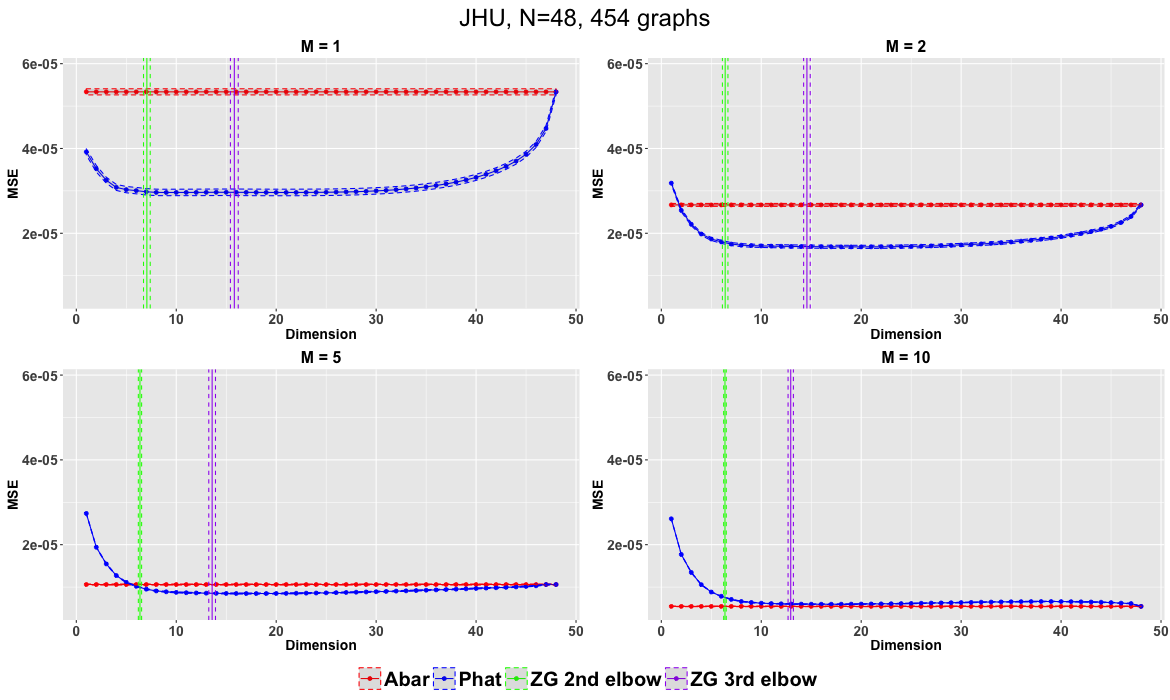
\includegraphics[width=14cm]{JHU.png}
\caption{Comparison of MSE between $\bar{A}$ (red) and $\hat{P}$ (blue) for JHU dataset while embedding the graphs into different dimensions with different size $M$ of the subsamples. The dimension chosen by Zhu and Ghodsi is denoted by solid lines (2nd elbow) and dashed lines (3rd elbow). When $M$ is small, $\hat{P}$ outperforms $\bar{A}$ with a flexible range of the embedding dimension including what Zhu and Ghodsi selects.}
\label{fig:JHU}
\end{figure}

\begin{figure}[!htb]
\centering
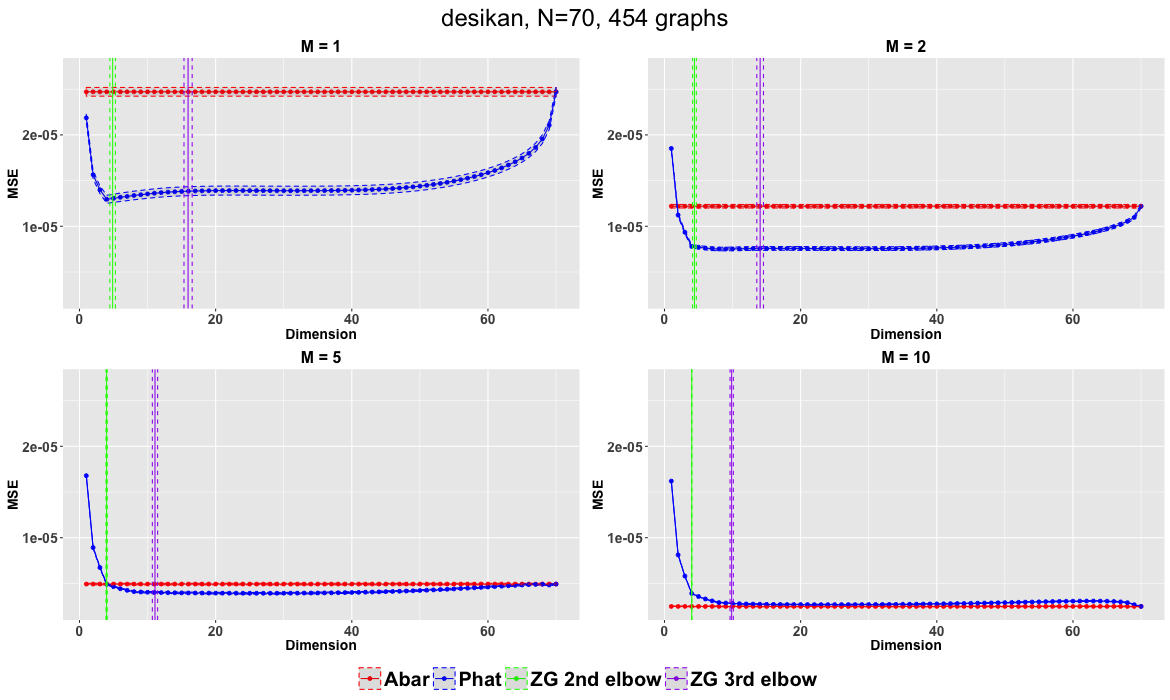
\includegraphics[width=14cm]{desikan.png}
\caption{Comparison of MSE between $\bar{A}$ (red) and $\hat{P}$ (blue) for desikan dataset while embedding the graphs into different dimensions with different size $M$ of the subsamples. The dimension chosen by Zhu and Ghodsi is denoted by solid lines (2nd elbow) and dashed lines (3rd elbow). When $M$ is small, $\hat{P}$ outperforms $\bar{A}$ with a flexible range of the embedding dimension including what Zhu and Ghodsi selects.}
\label{fig:desikan}
\end{figure}

\begin{figure}[!htb]
\centering
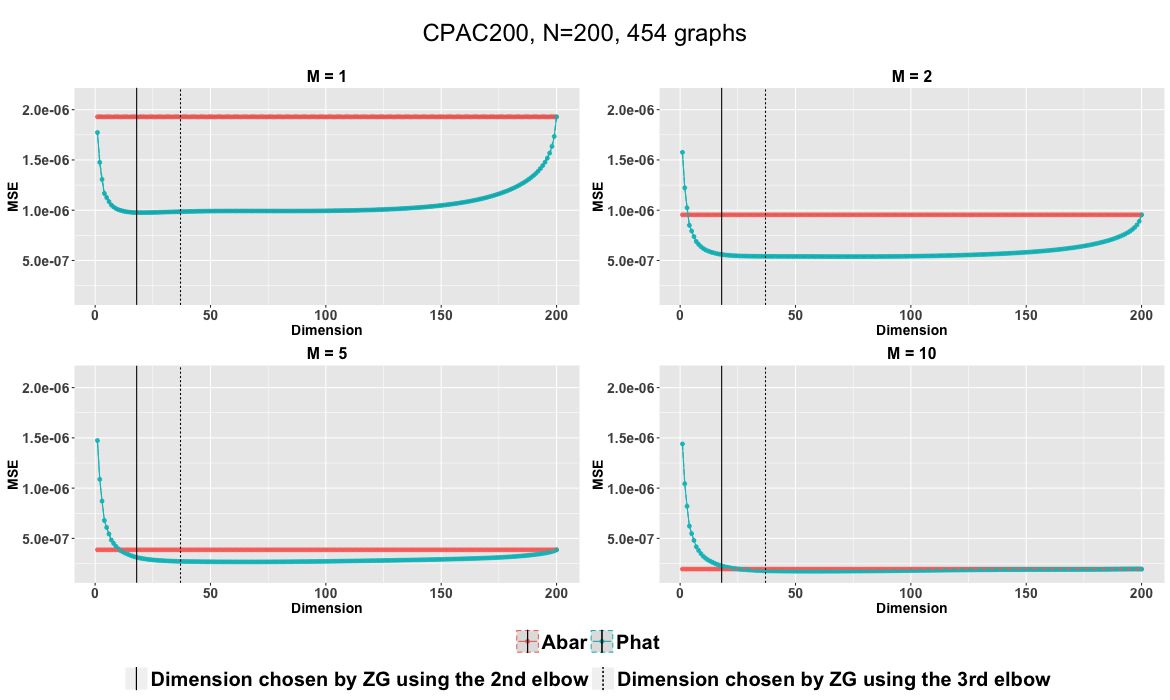
\includegraphics[width=14cm]{CPAC200.png}
\caption{Comparison of MSE between $\bar{A}$ (red) and $\hat{P}$ (blue) for CPAC200 dataset while embedding the graphs into different dimensions with different size $M$ of the subsamples. The dimension chosen by Zhu and Ghodsi is denoted by solid lines (2nd elbow) and dashed lines (3rd elbow). When $M$ is small, $\hat{P}$ outperforms $\bar{A}$ with a flexible range of the embedding dimension including what Zhu and Ghodsi selects.}
\label{fig:CPAC200}
\end{figure}





\newpage

